\chapter{Testování}



\section{Výsledky simulace}

Pomocí ROS 2 \textit{node} se nám podařilo posílat zprávy do simulovaného PX4 firmware a tím ovládat dron v \textit{offboard} letovém režimu. Na obrázku \ref{fig:SIM3} v levém horním rohu je zobrazené, že dron je v režimu \textit{offboard flight mode}. Obrázek \ref{fig:SIM4} zobrazuje simulační prostředí Gazebo 11 které poskytuje fyzikální model \uv{světa} a graficky zobrazuje aktuální stav objektů v robotické misi.

\begin{figure}[!ht]
  \begin{center}
    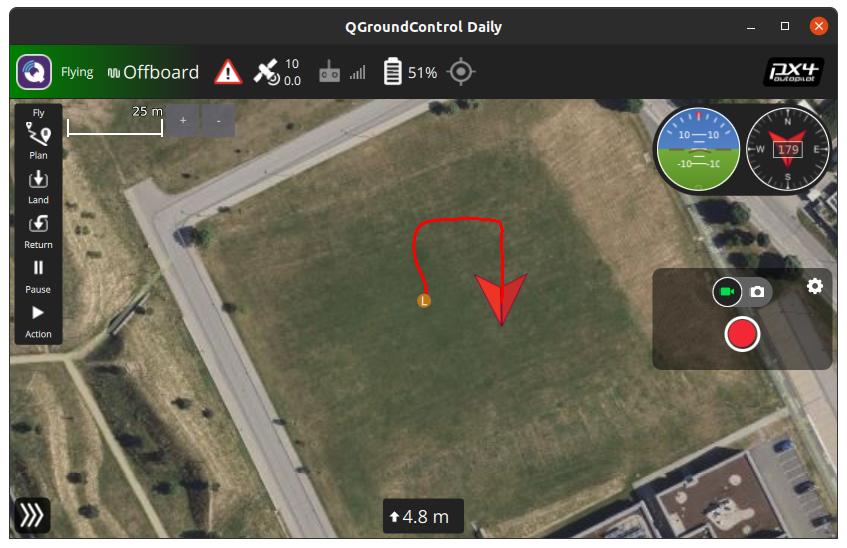
\includegraphics[scale=0.43]{obrazky/SIM3}
  \end{center}
  \caption[Software QGroundControl s dronem v \textit{offboard flight mode}]{Software QGroundControl s dronem v \textit{offboard flight mode}.}
  \label{fig:SIM3}
\end{figure}

\begin{figure}[!ht]
  \begin{center}
    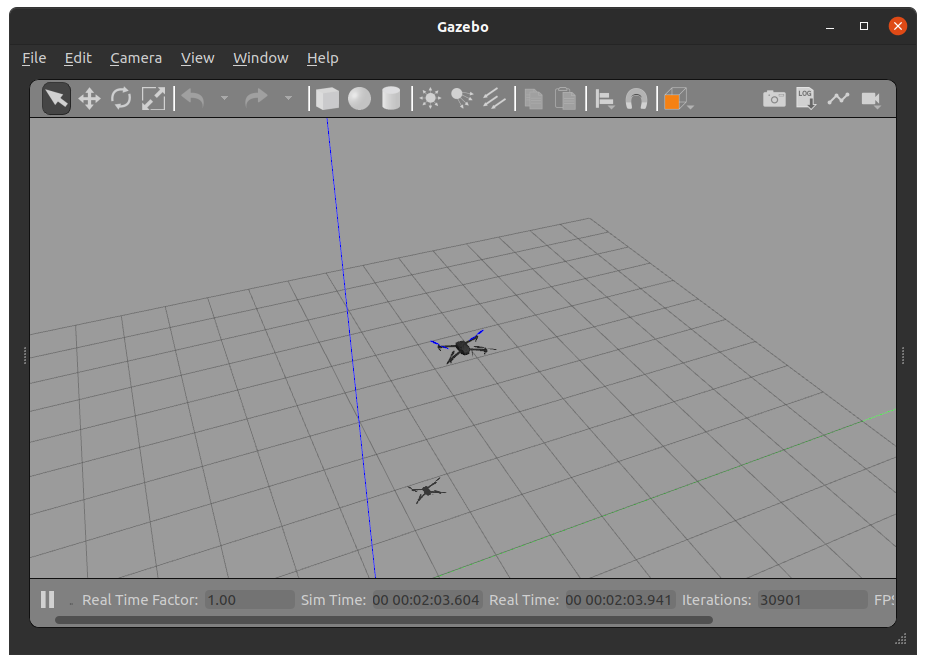
\includegraphics[scale=0.4]{obrazky/SIM4}
  \end{center}
  \caption[Bezpilotní mise v simulátoru Gazebo]{Bezpilotní mise v simulátoru Gazebo.}
  \label{fig:SIM4}
\end{figure}